% defines
\def\dispxi#1{\mathbb{D}_\xi^{#1}}
\def\mathbox#1{\fbox{$\displaystyle #1$}}

% main content

% Lecture 12  ---  21.04.21
\section{Інтервальні оцінки параметрів.}
Для того, щоб перейти до поняття інтервальної оцінки, нам знадобиться деякий теоретичний мінімум щодо розподілу числових характеристик гаусівських вибірок.
\subsection{Розподіли числових характеристик гаусівських вибірок.}
Нехай є Г.С.: $\xi \sim N(a, \sigma^2)$, що породжує вибірку $\xi_1, \dots , \xi_n$ --  незалежні, гаусівські.
\begin{itemize}
 \item Маємо  вибіркове середнє $\overline{\xi} = \frac{\xi_1 + \dots + \xi_n}{n} $.
  \item  Якщо правжнє математичне сподівання $a$ відоме: $ \mathbb{D}^*_\xi = \frac{1}{n}  \sum\limits_{i = 1}^{n}{(\xi_i - a)^2} $;
  \item Інакше можемо знайти $\mathbb{D}^{**}_\xi = \frac{1}{n}  \sum\limits_{i = 1}^{n}{(\xi_i - \overline{\xi})^2}$ або $\mathbb{D}^{***}_\xi = \frac{1}{n-1}  \sum\limits_{i = 1}^{n}{(\xi_i - \overline{\xi})^2}$.
\end{itemize}
\blue{Як розподілені ці характеристики?}
\subsubsection{Вибіркове середнє.}
За властивостями гаусівських величин: \mathbox{\overline{\xi}\sim N \left( a, \dfrac{\sigma^2}{2} \right)}.
\subsubsection{Вибіркова дисперсія.}
Нехай \textit{відоме} $\mathbb{E} \xi = a \Longrightarrow \displaystyle
\dispxi{*} : \ \
\frac{n \dispxi{*}}{\sigma^2} = \frac{n \frac{1}{n}  \sum\limits_{i = 1}^{n}{(\xi_i - a)^2}}{\sigma^2} =  \sum\limits_{i = 1}^{n}{ \left( \frac{\xi_i - a}{\sigma} \right)^2 } =  \sum\limits_{i = 1}^{n}{\tilde{\xi}^2_i} \sim \chi_n^2
$.
$$
\forall i : \xi_i \sim N(a, \sigma^2) \quad \Longrightarrow \quad \tilde{\xi}_i = \frac{\xi_i - a}{\sigma} \sim N(0, 1) \quad \Longrightarrow \quad \fbox{$\displaystyle \frac{n \dispxi{*}}{ \sigma^2} \sim \chi^2_n $}
$$
Нехай $\mathbb{E} \xi$ -- \textit{невідоме}. Тоді:
$$
\dispxi{**} = \frac{1}{n}  \sum\limits_{i = 1}^{n}{(\xi_i - \overline{\xi})^2} =
\frac{1}{n}  \sum\limits_{i = 1}^{n}{\xi_i^2}  -    \left( \frac{1}{n} \sum\limits_{i = 1}^{n}{\xi_i} \right)^2 = \overline{\xi^2} - (\overline{\xi})^2
$$
Спершу розглянемо величину коваріації між $\overline{\xi}$ та $\xi_i - \overline{\xi}$:
$$
\begin{gathered}
\mathrm{cov}(\overline{\xi}, \xi_i - \overline{\xi}) = \mathbb{E} \overline{\xi} \left( \xi_i - \overline{\xi} \right) - \mathbb{E} \overline{\xi} \cdot \underbrace{\mathbb{E}\left( \xi_i - \overline{\xi} \right)}_{= a-a = 0} =
\mathbb{E} \frac{\xi_1 + \dots + \xi_n}{n} \left( \xi_i - \frac{\xi_1 + \dots + \xi_n}{n} \right) =
\\
 = \mathbb{E} \left(  \frac{\xi_1 + \dots + \xi_n}{n} \cdot \xi_i  \right)- \mathbb{E} \left( \frac{\xi_1 + \dots + \xi_n}{n} \right)^2 = \mathbb{E} \frac{\xi_i^2}{n} +  \sum\limits_{j \neq i}^{}{ \frac{\xi_i \cdot \xi_j}{n} } -
\\
- \frac{1}{n^2} \left( \mathbb{E} \xi_1^2 + \dots + \mathbb{E}\xi_n^2 + 2 \mathbb{E}\xi_1 \xi_2 + \dots + 2 \mathbb{E} \xi_{n-1}\xi_n \right) = \left| \  \begin{gathered}
 \mathbb{E} \xi_i^2 - (\mathbb{E}\xi_i)^2 = \mathbb{D}\xi_i\\
 \mathbb{E} \xi_i^2 = a^2 + \sigma^2
\end{gathered} \  \right|  =
\\
=\frac{1}{n} (a^2 + \sigma^2)  \frac{n-1}{n} \cdot  a^2 + \frac{1}{n^2} (na^2 + n\sigma^2 - 2\frac{n(n-1)}{2}a^2 )=
\\
=
\frac{a^2}{n} + \frac{\sigma^2}{n} + a^2 -   \frac{a^2}{n} -   \frac{a^2}{n} - \frac{\sigma^2}{n}  -  a^2 +  \frac{a^2}{n} = \mathbf{0}
\end{gathered}
$$
Остаточно, отримали, що $\overline{\xi}$ не корелює з $\xi_i - \overline{\xi}\ \forall i.$ Тобто:
$$
\begin{gathered}
  \mathrm{corr} (\overline{\xi}, \xi_i - \overline{ \xi}) = 0 \quad \forall i\\
  \Downarrow\\
  \mathrm{corr} \left( \overline{\xi}, \begin{bmatrix}
   \xi_1 - \overline{\xi}\\
   \vdots\\
   \xi_n - \overline{\xi}
  \end{bmatrix} \right) = 0\\
  \text{За власт. } \Downarrow \ N(a, \sigma^2)\\
   \overline{\xi} \independent\begin{bmatrix}
    \xi_1 - \overline{\xi}\\
    \vdots\\
    \xi_n - \overline{\xi}
   \end{bmatrix}
\\
\Downarrow\\
\overline{\xi} \independent  \sum\limits_{i = 1}^{n}{ (\xi_i - \overline{\xi})^2} = \dispxi{**}
\\
\text{Для гаусівської Г.С. вибіркове середнє та вибіркова дисперсія \red{є незалежними}.}
\end{gathered}
$$
Повернемося до визначення розподілу вибіркової дисперсії:
$$
\dispxi{**} = \frac{1}{n}  \sum\limits_{i = 1}^{n }{ \xi_i^2} - \left( \frac{1}{n}  \sum\limits_{i =1 }^{ n}{ \xi_i}  \right)^2 \quad \Longrightarrow \quad
\frac{1}{n}  \sum\limits_{i = 1}^{n }{ \xi_i^2} = \dispxi{**}+
\left( \frac{1}{n}  \sum\limits_{i =1 }^{ n}{ \xi_i}  \right)^2
$$
$$
\frac{\xi_i - a}{\sigma} = \tilde{\xi}_i \longrightarrow \xi_i  \quad \qquad
\chi_n^2 \sim \sum\limits_{i = 1}^{n }{ \tilde{\xi}_i^2} =
\underbrace{n \mathbb{D}_{\tilde{\xi}}^{**}}_{\chi_{n-1}^2} +
\underbrace{\left( \frac{1}{\sqrt{n}}  \sum\limits_{i =1 }^{ n}{ \tilde{\xi}_i}  \right)^2}_{N(0, 1)^2 \sim \chi_1^2}
$$
В останньому міркуванні скористалися фактом незалежності, отриманим раніше:
$$
\overline{\xi} \independent \mathbb{D}_{\xi}^{**}  \quad \Longrightarrow \quad  \left( \frac{1}{\sqrt{n}}  \sum\limits_{i =1 }^{ n}{ \tilde{\xi}_i}  \right)^2 \ \independent \ n \mathbb{D}_{\tilde{\xi}}^{**}
$$
Таким чином, довели, що $ n \mathbb{D}_{\tilde{\xi}}^{**} \sim \chi_{n-1}^2$. Розпишемо:
$$
n \mathbb{D}_{\tilde{\xi}}^{**}  =
\sum\limits_{i = 1}^{n}{\left(  \tilde{\xi}_i - \frac{\tilde{\xi}_1 + \dots + \tilde{\xi}_n}{n} \right)^2 } \!\! =  \sum\limits_{i = 1}^{n}{
 \left(   \frac{\xi_i - a}{\sigma} - \frac{(\xi_1- a)  + \dots + (\xi_n - a)}{n\sigma} \right)^2
} =
$$
$$
= \frac{1}{\sigma^2} \sum\limits_{i = 1}^{n}{
 \left(   \xi_i - a   - \frac{\xi_1  + \dots + \xi_n}{n}+ \frac{an}{n} \right)^2} = \frac{n}{\sigma^2} \cdot \frac{1}{n}  \sum\limits_{i = 1}^{ n}{\left(  \xi_i - \overline{\xi} \right)^2} = \mathbox{ \frac{n}{\sigma^2} \cdot \mathbb{D}_{\xi}^{**}}
$$
\begin{boxteo}
  Остаточно, довели такі властивості:
  $$
    \begin{array}{l}
    \text{1) } \overline{\xi} \sim N \left( a, \dfrac{\sigma^2}{n} \right)\\
  \text{2) } \dfrac{n \cdot \mathbb{D}_{\xi}^{**} }{\sigma^2} \sim \chi^2_n
  \end{array} \qquad \qquad
  \begin{array}{l}
   \text{3) }  \dfrac{n \cdot \mathbb{D}_{\xi}^{**}}{\sigma^2} \sim \chi_{n-1}^2 \ \  \text{та } \  \dfrac{(n-1) \cdot \mathbb{D}_{\xi}^{***}}{\sigma^2} \sim \chi_{n-1}^2\\
    \text{4) } \overline{\xi} \independent \mathbb{D}_{\xi}^{**}
  \end{array}
  $$
\end{boxteo}
\begin{consequence} Розглянемо деякі наслідки з попередньої теореми:
$$
  \begin{array}{l}
  \text{1) }\sqrt{n} \dfrac{\overline{ \xi} - a}{\sigma} \sim N(0,1)\\
  \ \\
\text{2) } \dfrac{n \cdot \mathbb{D}_{\xi}^{*}}{\sigma^2} \sim \chi_n^2
\end{array} \qquad \qquad
\begin{array}{l}
 \text{3) }  \mathbox{\sqrt{n-1} \frac{\overline{\xi} - a}{\sqrt{\dispxi{**}}} \sim St_{n-1}}\\
 \ \\
  \text{4) } \dfrac{n \dispxi{**}}{\sigma^2} \sim \chi_{n-1}^2
\end{array}
$$
\end{consequence}
\newpage
\subsection{Інтервальні оцінки параметрів генеральної сукупності.}
Мотивація: існує суттєвий недолік точкових оцінок --- \blue{невідома їх точність.}
\begin{defo}
 Інтервал $(\theta^*_1, \theval_2)$ називають \red{довірчим інтервалом} для параметру $\theta$ з довірчою імовірністю (надійністю) $\gamma$, якщо
 $
 \mathbb{P} \left\lbrace (\theta^*_1, \theval_2) \ni \theta \right\rbrace = \gamma
 $.
 \end{defo}
 \begin{remark}[1]
   $\theta^*_1, \theval_2$ --  випадкові величини. $\theta$ -- невідоме конкретне число. Таким чином, розглядаємо ймовірність потрапляння у інтервал як функцію від $\theta^*_1(\overrightarrow{\xi}), \theval_2(\overrightarrow{\xi})$.
 \end{remark}
 \begin{remark}[2]
 Зазвичай $\gamma = 0.9, 0.95, 0.99$. $(\theta^*_1, \theval_2)\xrightarrow[\gamma \to 1]{}  (-\i, +\i)$
 \end{remark}
\subsubsection{Знаходження точних довірчих інтервалів для гаусівської Г.С.}
\begin{enumerate}
  \item Інтервал для $\mathbb{E} \xi = a$ при відомій дисперсії:
  $$
  \sqrt{n} \dfrac{\overline{ \xi} - a}{\sigma} \sim N(0,1) \quad \Longrightarrow \quad
  \begin{gathered}
  \setlength{\fboxrule}{0.0pt}
  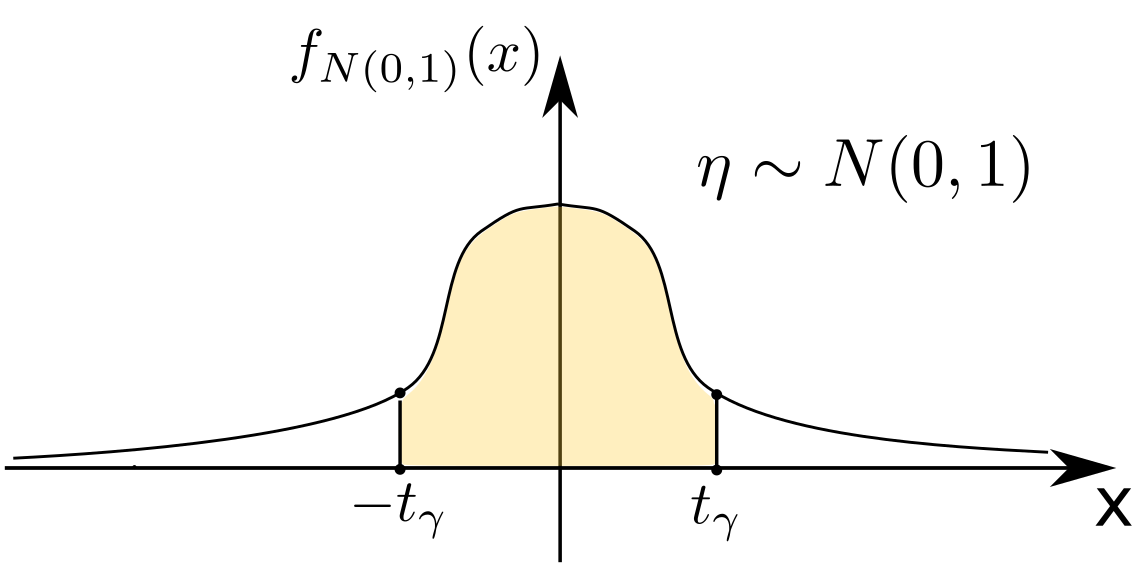
\includegraphics[scale=0.18]{assets/lectures_part_6-25d71e2a.png}
  \end{gathered}
  $$
  $$
  \gamma = \mathbb{P} \left\lbrace \eta \in (-t_{\gamma}, t_{\gamma}) \right\rbrace = \Laplas \left( t_{\gamma}  \right)  - \Laplas(- t_{\gamma}) = 2\Laplas \left( t_{\gamma} \right) \Longrightarrow \mathbox{t_{\gamma} = \Laplas^{-1}\left( \frac{\gamma}{2} \right) }
  $$
  $$
  \gamma = \mathbb{P} \left\lbrace   \sqrt{n} \dfrac{\overline{ \xi} - a}{\sigma} \in (-t_{\gamma}, t_{\gamma}) \right\rbrace \quad \Longrightarrow \quad \mathbox{
  \overline{\xi} - \frac{\sigma t_{\gamma}}{\sqrt{n} } < a < \overline{\xi} +  \frac{\sigma t_{\gamma}}{\sqrt{n} }
  }
  $$
  \item Інтервал для дисперсії при відомому $\mathbb{E} \xi = a$:
  $$
   \dfrac{n \cdot \mathbb{D}_{\xi}^{*}}{\sigma^2} \sim \chi_n^2 \quad \Longrightarrow \quad \begin{gathered}
   \text{Аналогічно, визначаємо інтервал на PDF:}\\
   \eta \sim \chi^2_n : \mathbb{P} \left\lbrace t_{\frac{1 + \sigma}{2}} < \eta < t_{\frac{1 - \sigma}{2}}  \right\rbrace
   \end{gathered}
  $$
  $$
  t_{\frac{1 + \sigma}{2}} <  \dfrac{n \cdot \mathbb{D}_{\xi}^{*}}{\sigma^2} < t_{\frac{1 - \sigma}{2}}
 \quad \Longrightarrow \quad
 \mathbox{ \dfrac{n \cdot \mathbb{D}_{\xi}^{*}}{t_{\frac{1 - \sigma}{2}}}  < \sigma^2 < \dfrac{n \cdot \mathbb{D}_{\xi}^{*}}{ t_{\frac{1 + \sigma}{2}} }
 }\qquad t   \text{ -- для розподілу } \chi_n^2
  $$
  \item Інтервал для дисперсії при невідомому $\mathbb{E} \xi$:
  $$
  \dfrac{n \dispxi{**}}{\sigma^2} \sim \chi_{n-1}^2  \quad \Longrightarrow \quad
  \mathbox{ \dfrac{n \cdot \mathbb{D}_{\xi}^{*}}{t^{(n-1)}_{\frac{1 - \sigma}{2}}}  < \sigma^2 < \dfrac{n \cdot \mathbb{D}_{\xi}^{*}}{ t^{(n-1)}_{\frac{1 + \sigma}{2}} }
  }\qquad  t^{(n-1)} \text{ -- для розподілу } \chi_{n-1}^2
  $$
  \item Інтервал для $\mathbb{E} \xi = a$ при невідомій дисперсії:
  $$
  \sqrt{n-1} \frac{\overline{\xi} - a}{\sqrt{\dispxi{**}}} \sim St_{n-1} \quad \Longleftarrow \quad \begin{gathered}
\text{Знов користуємося наслідком теореми 5.1 та }\\
\text{визначаємо інтервал на } f_{St_{n-1}} (x)
  \end{gathered}
  $$
  $$
  - t_{\gamma}  < \frac{\sqrt{n-1} \cdot (\overline{ \xi} - a )}{\sqrt{\mathbb{D}_{\xi}^{**}}} < t_{\gamma} \quad \Longrightarrow \quad \mathbox{
\overline{\xi} - \frac{t_{\gamma}\sqrt{\mathbb{D}_{\xi}^{**}}}{\sqrt{n-1}} < a < \overline{\xi} + \frac{t_{\gamma}\sqrt{\mathbb{D}_{\xi}^{**}}}{\sqrt{n-1}}
  }
  $$
  де  $t_{\gamma}$ -- для розподілу Стьюдента з $n-1$ ступенями вільності.
\end{enumerate}
\subsubsection{Точні довірчі інтервали для будь-яких розподілів. }
\begin{center}
 \large Загальний алгоритм пошуку точних довірчих інтервалів.
\end{center}
\begin{enumerate}
  \item Знайти таку функцію $H(\overrightarrow{x}, \theta)$, що:
  \begin{itemize}
    \item $H(\overrightarrow{\xi}, \theta)$ -- розподіл цієї величини не залежить від $\theta$.
    \item $\exists H^{-1} : \theta = H^{-1}(\overrightarrow{\xi})$.
  \end{itemize}
  \item $H(\overrightarrow{\xi}, \theta)$ -- розподіл не залежить від $\theta \ \Longrightarrow \
  \gamma = \mathbb{P} \left\lbrace t_1 < H(\overrightarrow{\xi}, \theta) < t_2 \right\rbrace
  $.
  \item Розв'язуємо відносно $\theta$. Отримаємо: $\theta_1^* (\overline{\xi}) < \theta < \theta_2^* (\overline{\xi})$.
\end{enumerate}
\newpage
\subsubsection{Асимптотичны довірчі інтервали.}
\begin{defo}
 $(\theval_{1,n} , \theval_{2,n})$ називається \red{асимптотичним довірчим інтервалом}, якщо:
$$
 \lim\limits_{n\to  \infty}{\mathbb{P} \left\lbrace  \theval_{1,n} < \theta < \theval_{2,n} \right\rbrace} = \gamma
$$
\end{defo}
\begin{center}
 \large Алгоритм пошуку асимптотичного довірчого інтервалу.
\end{center}
\begin{enumerate}
  \item $\theval$ -- точкова оцінка, яка є асимптотично нормальною (наприклад, містить суми незалежних однаково розподілених випадкових величин).
  \item $\displaystyle \frac{ \theval - \mathbb{E} \theval}{
  \sqrt{\mathbb{D} \theval}
  } \approx N(0,1) $ при великих $n$. Шукаємо симетричний довірчий інтервал:
  $$
  \Laplas (t_{\gamma}) = \Laplas(t_{\gamma}) - \Laplas(0) =  \frac{\gamma}{2} \quad \Longrightarrow \quad t_{\gamma} : \Laplas(t_{\gamma}) = \frac{\gamma}{2}
  $$
  $$
  \mathbb{P} \left\lbrace - t_{\gamma} < N(0,1) < t_{\gamma} \right\rbrace = \gamma \quad \Longrightarrow \quad  \mathbox{  \mathbb{P} \left\lbrace - t_{\gamma} <\frac{ \theval - \mathbb{E} \theval}{
  \sqrt{\mathbb{D} \theval}
  } < t_{\gamma} \right\rbrace \approx \gamma}
  $$
  \item Розв'язуючи цю нерівність відносно $\theta$, отримаємо асимптотичний довірчий интервал для $\theta$.
\end{enumerate}
\newpage



\section{
Статистичні гіпотези. Перевірка гіпотез.
}
\begin{defo}
 \red{Статистична гіпотеза} --- це довільне припущення про розподіл Г.С. або його параметри, яке можна перевірити на основі вибіркових даних.
\end{defo}
\begin{multicols}{2}
\begin{itemize}
  \item  \blue{Непараметрична гіпотеза} --- це твердження, про розподіл Г.С. Приклад: $H_0$  -- гаусівська.
  \item \blue{Параметрична гіпотеза} --- це твердження про параметри Г.С. \\ Приклад:$H_0 = Pois(\lambda)$.
  \item \blue{Проста гіпотеза} --- це гіпотеза, що повністю визначає розподіл Г.С. або його параметри.
  \item \blue{Складна гіпотеза} --- стверджує про належність Г.С. до певного сімейства розподілів.
\end{itemize}
\end{multicols}

Розглянемо $H_0$ -- \textit{основна гіпотеза}. Якщо ж $H_0$ не виправдовується, то ми приймаємо \textit{альтернативну гіпотезу} -- $H_1$ і відхиляємо $H_0$.
\begin{defo}
 \red{Статистичний критерій} --- процедура, яка на основі вибіркових даних дозволяє або прийняти $H_0$ , або відхилити $H_0$ і прийняти $H_1$.
\end{defo}
\begin{example}
  Нехай є вибірка $\xi_1 , \dots , \xi_n$, $H_0$ -- основна гіпотеза, $H_1$ -- альтернативна. \par
     Вибираємо статистику $T(\xi_1, \dots , \xi_n)$ та простір змагань $\mathbb{R}^n (\xi_1, \dots, \xi_n)$:
     \begin{center}
     \vspace*{-1em}
     \setlength{\fboxrule}{0.0pt}
   
\includegraphics[scale=0.3]{assets/lectures_part_6-b1580c4d.png}
     \end{center}
  Головне питання буде полягати у виборі зазначених на малюнку областей. Вони будуть визначатися задопомогою обраної статистики. \par Припустимо: за умови виконання $H_0 : T(\xi_1, \dots, \xi_n)$ з великою імовірністю потрапляє в деяку область. Якщо статистика $T$ потрапляє в область $\omega \Rightarrow$ приймаємо $H_0$.
  \end{example}
  \textit{Розглянемо більш конкретний приклад.} Маємо: Г.С. $\xi \sim N(a,\sigma^2),
  \  \sigma $ -- відома.
  $$
   H_0 = \left\lbrace a = a_0 \right\rbrace\qquad
   H_1 = \left\lbrace a = a_1 \right\rbrace
   \qquad a_0 < a_1
   $$
$$
T(\xi_1 , \dots , \xi_n) = \frac{\xi_1 + \dots + \xi_n}{n} = \overline{\xi}
$$
Таким чином, оберемо $x \in (a_0, a_1)$ так, що:
\begin{itemize}
  \item Якщо $\overline{\xi} \leq  x$: приймаємо $H_0 \Rightarrow \omega = \left\lbrace \overline{y} \in \mathbb{R}^n : \overline{y} \leq x  \right\rbrace$.
  \item Якщо $\overline{\xi}>  x$: приймаємо $H_1 \Rightarrow \overline{\omega} = \left\lbrace \overline{y} \in \mathbb{R}^n : \overline{y} > x  \right\rbrace$.
\end{itemize}
\subsection{Помилки І-го та ІІ-го роду.}
\begin{center}
\vspace*{2em}
 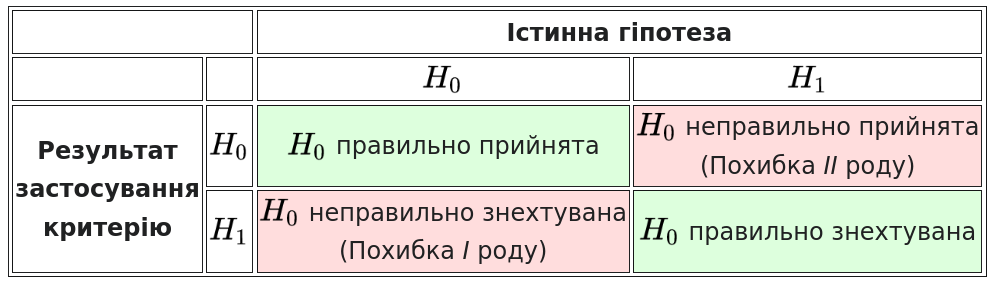
\includegraphics[scale=0.3]{assets/lectures_part_6-4c5b9490.png}
\end{center}
\vspace*{1em}
\begin{itemize}
  \item Якщо \textit{істинна} гіпотеза помилково відкидається, то ця помилка називається \red{помилкою першого роду} (англ. type I errors $\alpha$ errors, \blue{false positives}).
  \item Якщо помилково приймається \textit{хибна} гіпотеза - це \red{помилка другого роду} (англ. type II errors $\beta$ errors, \blue{false negatives}).
\end{itemize}
\subsubsection{Влучність та повнота (Precision and recall).}
\vspace*{-1em}
В розпізнаванні образів, інформаційному пошуку та класифікації широко застосовуються дві метрики, які відображають наявність помилок першого і другого роду.
\begin{defo}
\red{Влучність} (англ. precision, яку також називають прогностичною значущістю позитивного результату) є часткою релевантних зразків серед знайдених.
\end{defo}
\begin{defo}
  \red{Повнота} (англ. recall, відома також як чутливість) є часткою загального числа позитивних зразків, яку було дійсно знайдено.
\end{defo}
Влучність не слід плутати з \blue{точністю} (англ. accuracy), яка є часткою правильно спрогнозованих результатів, як позитивних, так і негативних.
$$
\vspace*{-1em}
\begin{gathered}
\setlength{\fboxrule}{0.0pt}
 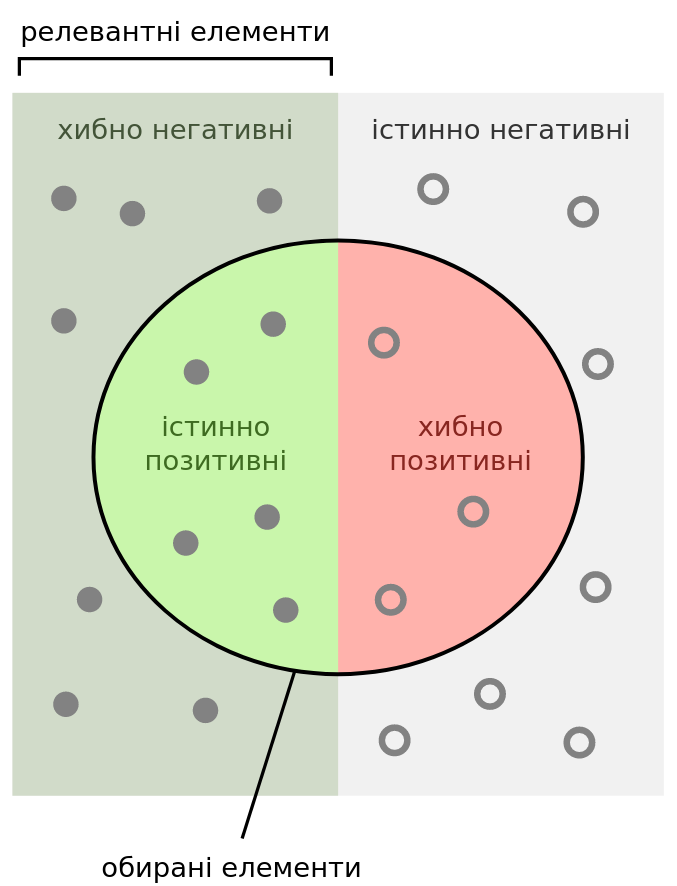
\includegraphics[scale=0.25]{assets/lectures_part_6-79981811.png}
 \end{gathered}
 \qquad
 \begin{gathered}
 \setlength{\fboxrule}{0.0pt}
 
\includegraphics[scale=0.4]{assets/lectures_part_6-304942b8.png}
 \end{gathered}
 \vspace*{0.1em}
$$
\subsubsection{Рівень значущості та потужність критерію.}
\vspace*{-1em}
\begin{spacing}{1}
\blue{Рівень значущості критерію} --- це ймовірність помилки І-го роду:
  $$
  \mathbb{P} \left\lbrace \text{Приймаємо } H_1 \ \big| \  H_0 \text{ -- вірна} \right\rbrace = \mathbb{P} \left\lbrace \overrightarrow{\xi} \in \overline{\omega}\ \big| \  H_0 \text{ -- вірна} \right\rbrace = \alpha
  $$
\blue{Потужність критерію} дорівнює $(1 - \beta), $ де $\beta$ -- ймовірність помилки ІІ-го роду:
  $$
  \mathbb{P} \left\lbrace \text{Приймаємо } H_1 \ \big| \  H_1 \text{ -- вірна} \right\rbrace = \mathbb{P} \left\lbrace \overrightarrow{\xi} \in \omega\ \big| \  H_1 \text{ -- вірна} \right\rbrace = \beta
  $$
\end{spacing}
\textit{Повернемося до прикладу.} Саме від значущості та потужності критерію буде залежати положення ``межі'' $x$. Найчастіше вибирають значення: $\alpha = 0.01, 0.05, 0.1$.\par
Зафіксуємо рівень значущості $\alpha = 0.05$ та побудуємо критерій (знайдемо $x$).
$$
\alpha = \mathbb{P} \left\lbrace \overrightarrow{\xi} \in \overline{\omega} \  \big| \  H_0 \right\rbrace = \mathbb{P} \left\lbrace  \overline{\xi} > x  \  \big| \  a = a_0 \right\rbrace  =
$$
$$
=
\left| \begin{gathered}
 a = a_0 \Longrightarrow
 \xi_1 , \dots , \xi_n \sim N(a_0, \sigma^2)\\
 \Downarrow \\
 \overline{ \xi} = \frac{\xi_1 , \dots , \xi_n}{n}   \sim N(a_0, \sigma^2/n)
\end{gathered} \right| = \frac{1}{2} - \Laplas \left(  \sqrt{n} \frac{x - a_0}{\sigma}  \right) = \frac{1}{2} - \alpha
$$
$$
 \sqrt{n} \frac{x - a_0}{\sigma}= t_{\alpha}\quad \Longrightarrow \quad \mathbox{x = a_0 + \frac{\sigma t_{\alpha}}{\sqrt{n}} }
$$
$$
1 - \beta = 1 - \mathbb{P} \left\lbrace \overrightarrow{\xi} \in \omega \ \big| \  H_1 \right\rbrace  =
1 - \mathbb{P} \left\lbrace \overrightarrow{\xi} \in \omega \ \big| \  a= a_1 \right\rbrace = \frac{1}{2} + \Laplas \left( \sqrt{n} \cdot \frac{a_1 - x}{ \sigma}  \right)
$$
Бачимо, що збільшуючи $\alpha$ збільшуємо і $\beta$: \mathbox{\alpha \downarrow  \Rightarrow t_{\alpha}\to \infty \Rightarrow \beta \uparrow \Rightarrow (1- \beta) \downarrow}. \par
Знайдемо рівень значущості та потужність критерію для загального випадку:
\[
\begin{split}
\alpha &= \mathbb{P} \left\lbrace  \overrightarrow{\xi} \in \overline{\omega} \ \big| \  H_0 \right\rbrace =
\infint{\begin{gathered}
 \overline{\omega}
\end{gathered}}  f_{\overline{\xi} }(x_1, \dots, x_n) \mathrm{d} x_1 \dots \mathrm{d} x_n =
\\ &=
\infint{\begin{gathered}
 \overline{\omega}
\end{gathered}}   \underbrace{f_{\xi}(x_1) \cdot \dots \cdot f_{\xi}(x_n)}_{\mathcal{L}_{H_0}(\overrightarrow{x})}\mathrm{d} x_1 \dots \mathrm{d} x_n =
\underset{\begin{gathered}
 \overline{\omega}
\end{gathered}}{\int\!\cdots\!\int}
\mathcal{L}_{H_0}(\overrightarrow{x})
\mathrm{d} x_1 \dots \mathrm{d} x_n
\end{split}
\]
Аналогічно, для потужності критерію:
\(
\
\displaystyle
\beta = \underset{\begin{gathered}
 \omega
\end{gathered}}{\int\!\cdots\!\int}
\mathcal{L}_{H_1}(\overrightarrow{x})
\mathrm{d} x_1 \dots \mathrm{d} x_n
\)\\
Зробимо висновок щодо прийняття чи відхилення гіпотези $H_0$:
\begin{itemize}
  \item Більш категоричний факт -- \blue{відхилення гіпотези} $H_0$: на рівні значущості $\alpha$, гіпотеза $H_0$ \textit{суперечить} вибірковим даним.
  \item \blue{Прийняття} $H_0$:\  -//- $H_0$ \textit{не суперечить} вибірковим даним.
\end{itemize}
\subsection{Критерії згоди (goodness-of-fit).}
Припустимо, є Г.С. та вибірка з неї: $\overrightarrow{ \xi} = (\xi_1, \dots, \xi_n)$. \par
Нехай $F$ -- теоретична функція розподілу $\xi$. Висуваємо гіпотезу:
$$
H_0 = \left\lbrace F(x) = F_0(x) \right\rbrace \qquad \quad H_1 = \left\lbrace F(x) \neq  F_0(x) \right\rbrace
$$
\subsubsection{Критерій \(\chi^2\) (критерій Пірсона).}
\begin{itemize}
  \item Розіб'ємо область значень Г.С. \( \mathcal{E}_\xi \) на інтервали $\Delta_1, \Delta_2, \dots, \Delta_m:$
  \[
   \begin{dcases}
    \Delta_i \cap \Delta_j = \emptyset \quad \forall i \neq j \\
    \bigcup_i \Delta_i =  \mathcal{E}_\xi
   \end{dcases}
  \]
\end{itemize}
Складаємо таблицю. Наведемо опис застосованих характеристик:
\begin{enumerate}
  \item Кількість елементів, що потрапили в $\Delta_k = n_k$;
  \item Середня кількість елементів, що потрапили в $\Delta_k$, якщо розподіл вгаданий правильно, тобто:
  \( \mathbb{E} \) (кількість елементів вибірки в \( \Delta_k \)) \(  = \mathbb{E} \mathrm{Bin}(n, \underbrace{\mathbb{P} \left\lbrace \xi \in \Delta_k \  \big| \  H_0 \right\rbrace}_{= p_k}) \)
\end{enumerate}
\[
 \begin{array}{l|c|c|c|c|c|c}
\text{Характеристики}   & \quad \Delta_1 \quad & \quad \Delta_2 \quad & \quad \cdots \quad & \quad \Delta_k \quad &\quad  \cdots \quad &\quad  \Delta_m \quad \\
\hline
1.\ n_k = \mathrm{card} \left\lbrace x_i \  \big| \   x_i \in \Delta_k \right\rbrace& n_1 &n_2 & \cdots & n_k& \cdots & n_m\\
\hline
2.\ \mathbb{E} n_{k, H_0}  = \mathbb{E} \mathrm{Bin}(n, p_k) = np_k
& np_1 &np_2 & \cdots & np_k& \cdots & np_m
 \end{array}
\]

\textbf{Головне завдання} може бути сформульовано наступним чином: наскільки близькими є \textit{реальні спостереження} (І рядок) до отриманих за припущенням (ІІ рядок).
Можемо використовувати для порівняння: \(  \sum\limits_{k=1}^{m}{ \frac{(n_k - np_k)^2}{np_k}} = \chi^2(n)\)
\begin{boxteo}[Пірсона про критерій \( \chi^2 \)]
 Якщо гіпотетичний розподіл вгадано правильно (тобто, \( H_0 \) справдовується), то:
 $$
 \chi^2 (n) \xrightarrow[\mathrm{d}]{n \to \i} \chi^2_{m-1}
 $$
 \textbf{Вправа:} Довести.
\end{boxteo}
\subsubsection{Застосування критерію \( \chi^2 \) для перевірки гіпотез.}
Якщо \( H_0 \) виконана, то за теоремою при великих \( n \ : \
\chi^2(n) \text{ має розподіл приблизно } \chi^2_{m-1}\). \par
Припустимо, що \(  \chi^2  > \chi_{m-1, \alpha}^2 \). Розглянемо можливі причини:
\begin{enumerate}
  \item Відбулася рідкісна подія ймовірності \( \alpha \); при цьому гіпотеза \( H_0 \) виконується, але є помилково відхиленною \( \Longrightarrow  \) виникає помилка І-го роду.
  \item Гіпотеза \( H_0 \) не виконується \( \Longrightarrow   H_0 \) відхиляємо, приймаємо \( H_1 \).
\end{enumerate}
Запишемо вимоги до $n, p_k$. Дані умови є суто практичними та можуть відрізнятися:
\[
 \begin{gathered}
  \forall k \in \overline{1, m}\\
np_k \geq 5
 \end{gathered} \qquad\quad \begin{cases}
  m \geq 20 \\
  np_k \geq  5
 \end{cases}
 \qquad \quad
 \begin{cases}
  m \leq 20 \\
  np_k \geq  10
 \end{cases}
\]
